%%%%%%%%%%%%%%%%%%%%%%%%%%%%%%%%%%%%%%%%%%%%%%%%%%%%%%%%%%%%%%%%%%%%%%%%%
% Antes de correr el código:
% 1. Ingresar al Menu
% 2. Cambiar la opción "Compiler" a XeLaTeX
% 3. Cambiar la opción "TeX live version" a 2020 (opacidad de la imagen)
%%%%%%%%%%%%%%%%%%%%%%%%%%%%%%%%%%%%%%%%%%%%%%%%%%%%%%%%%%%%%%%%%%%%%%%%%
\documentclass[10pt]{article}
\usepackage[T1]{fontenc}
\usepackage[utf8]{inputenc}
\usepackage[english]{babel}
\usepackage{listings}
\lstset{language=R}
\usepackage[a4paper]{geometry}
\usepackage[dvipsnames]{xcolor}
\usepackage[framemethod=TikZ]{mdframed}
\usepackage{graphicx,tikz}
\usepackage{array}
\usepackage{float}
\usepackage{tocloft}
\setlength{\cftsecnumwidth}{2em}

\geometry{top=2.54cm, bottom=2.54cm, left=2.54cm, right=2.54cm}

\usepackage{url}
\usepackage{lipsum} 
\usepackage{wrapfig}
\usepackage{subcaption}
\usepackage{multicol}

%==========================================
%======     FUENTE PARA CÓDIGOS      ======
%==========================================
\definecolor{codegreen}{rgb}{0,0.6,0}
\definecolor{codegray}{rgb}{0.1,0.1,0.1}
\definecolor{backcolour}{rgb}{0.98,0.98,0.98}

\lstdefinestyle{mystyle}{
  backgroundcolor=\color{backcolour},   
  commentstyle=\color{codegreen},
  keywordstyle=\color{blue},
  numberstyle=\tiny\color{codegray},
  stringstyle=\color{codegreen},
  basicstyle=\ttfamily\footnotesize,
  breakatwhitespace=false,         
  breaklines=true,                 
  captionpos=b,                    
  keepspaces=true,                 
  numbers=left,                    
  numbersep=5pt,                  
  showspaces=false,                
  showstringspaces=false,
  showtabs=false,                  
  tabsize=2
}

%==========================================
%==========     ESTILO TITLE     ==========
%==========================================
\newcommand{\City}[1]{\def\City{#1}}

\makeatletter         
\renewcommand\maketitle{
\begin{flushleft}
{\textcolor{black}{\huge \bfseries \@title }}\\[1ex]
\rule{\textwidth}{0.6pt}\\
\end{flushleft}
\vspace{-0.5cm}

\begin{flushleft}
\textcolor{black}{{\large  \@author} }\\[2ex]
\end{flushleft} } % Note the extra }
\makeatother

%==========================================
%==========    ESTILO CAPTION    ==========
%==========================================
\usepackage{caption}
\captionsetup[table]{name=Tabla ,textfont={it}, labelfont={bf},
                     justification=centering,
                     width =\dimexpr \textwidth-0.5cm\relax}
\captionsetup[figure]{textfont={it}, labelfont={bf},
                      justification=centering, skip=2pt,
                      belowskip=-5pt}
                      
%==========================================
%==========     ESTILO ITEM      ==========
%==========================================
\renewcommand{\labelitemi}{$\bullet$} 
\renewcommand{\labelitemii}{$\circ$} 
\renewcommand{\labelitemiii}{$\cdot$} 

%==========================================
%===    LINKS (Agregar Hyperlinks)     ====
%==========================================
\usepackage[style=apa,
            urldate=long]{biblatex} 
\addbibresource{Bib.bib}

\DeclareSourcemap{
  \maps[datatype=bibtex]{
    \map{
      \step[fieldsource=note, final]
      \step[fieldset=addendum, origfieldval, final]
      \step[fieldset=note, null]}
      }
}

\DefineBibliographyStrings{english}{urlseen = {Accessed }    
}

\usepackage[colorlinks=true,linkcolor=RoyalBlue,
            citecolor=RoyalBlue,urlcolor=RoyalBlue]{hyperref}

%==============================================================
%==============================================================
\title{ }

%%%%%%%%%%%%%%%%%%%%%%%%%%%%%%%%%%%%%%%%%%%%%%%%%%%%%%%%%%%%%%%
%%%%%%%%%%%%                 INICIO                %%%%%%%%%%%% 
%%%%%%%%%%%%%%%%%%%%%%%%%%%%%%%%%%%%%%%%%%%%%%%%%%%%%%%%%%%%%%%
\begin{document}

\begingroup
\let\clearpage\relax % prevent extra page breaks
\thispagestyle{empty}
\begin{center}
{\huge \bfseries Universidad de los Andes}

\vspace{25pt}
{\LARGE \bfseries Departamento de Ingeniería de Sistemas}

\vspace{15pt}

\includegraphics[width=100pt]{images/logo.png} 

\vspace{35pt}
{\LARGE \bfseries Laboratorio \#2: Análisis De Protocolos De La Capa De Aplicación}
\vspace{55pt}

{\Large \bfseries ISIS3204 - Infraestructura de Comunicaciones}


\vspace{100pt}
{\Large \bfseries Grupo 3: }

\end{center}

\begin{flushleft}
  \setlength{\parskip}{0pt}
  \setlength{\itemsep}{0pt}
  \hspace*{4cm}\large\bfseries Juan Esteban Quiroga - 202013216

  \hspace*{4cm}\large\bfseries Juan Manuel Rodriguez - 202013372

  \hspace*{4cm}\large\bfseries Andres Felipe Ortiz - 201727662
\end{flushleft}

\begin{center}
\vspace{60pt}

\Large\bfseries 2025-10
\end{center}

\mbox{}
\endgroup

\clearpage

\tableofcontents
\clearpage


\renewcommand{\thesection}{\arabic{section}}
\section*{Introducción}
\addcontentsline{toc}{section}{Introducción}
Lorem ipsum dolor sit amet, consectetur adipiscing elit. Sed nec tristique eros. Vestibulum ante ipsum primis in faucibus orci luctus et ultrices posuere cubilia curae; Pellentesque sit amet purus a sapien porta viverra. Cras in feugiat nisl. Mauris volutpat lorem in ligula dapibus, non aliquam eros tristique. Suspendisse potenti. Nunc laoreet augue ac viverra dictum. Integer mattis magna in nisi consequat, nec vehicula nulla dignissim. Ut nec aliquam libero. Sed eu nisl vitae mauris congue eleifend at nec urna.

%==============================================================
%=====================   8.1   ================================
%==============================================================
\renewcommand{\thesection}{8.\arabic{section}}
\setcounter{section}{0}
\section{Prueba ping}

Lorem ipsum dolor sit amet, consectetur adipiscing elit. Sed nec tristique eros. Vestibulum ante ipsum primis in faucibus orci luctus et ultrices posuere cubilia curae; Pellentesque sit amet purus a sapien porta viverra.


\begin{figure}[H]
    \centering
    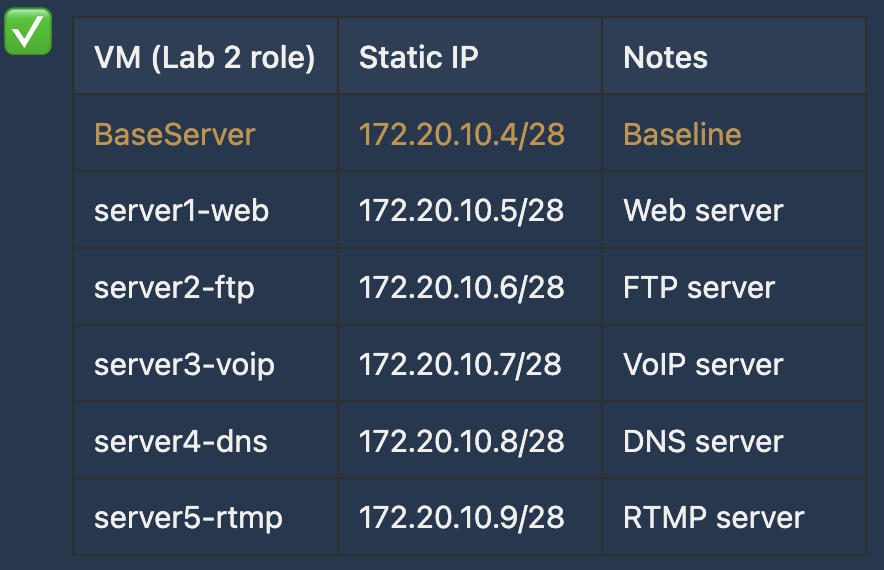
\includegraphics[width=0.65\textwidth]{lab-02-screenshots/server-ips.png}
    \caption{Configuración de IPs estáticas}
\end{figure}


\subsection{Prueba de conectividad al servidor DNS}
\subsection{Prueba de conectividad al servidor FTP}


%==============================================================
%=====================   8.2   ================================
%==============================================================
\renewcommand{\thesection}{8.\arabic{section}}
\section{Análisis de tráfico del Servicio DNS}
\subsection{Prueba de conectividad al Servidor Web (IP)}
\subsection{Prueba de conectividad al Servidor Web (URL)}


%==============================================================
%=====================   8.3   ================================
%==============================================================
\renewcommand{\thesection}{8.\arabic{section}}
\section{Análisis de tráfico del Servicio FTP}
\subsection{Conexión al servidor FTP}
\subsection{Descarga de archivo (Download)}
\subsection{Carga de archivo (Upload)}

%==============================================================
%=====================   8.4   ================================
%==============================================================
\renewcommand{\thesection}{8.\arabic{section}}
\section{Análisis de tráfico del Servicio Web}
\subsection{Acceso al servidor web mediante HTTP}

%==============================================================
%=====================   8.5   ================================
%==============================================================
\renewcommand{\thesection}{8.\arabic{section}}
\section{Análisis del protocolo HTTPS realizando navegación en el sitio de YouTube}

\subsection{Navegación en YouTube}
Se realizó la captura de tráfico mientras se navegaba en \textbf{https://www.youtube.com/}. 
Para reducir interferencias, se mantuvo una única pestaña activa en el navegador; se inició sesión con cuenta de Google y se realizaron acciones de navegación/comentarios. 
La captura se guardó como \texttt{YouTube\_view.pcapng}.

\begin{itemize}
    \item \textbf{Filtro aplicado en Wireshark:} \texttt{tcp.port == 443}.
    \item \textbf{Capa de aplicación (TLS):} Se observan mensajes del \textit{handshake TLS} (\textit{Client Hello}, \textit{Server Hello}, \textit{Certificate}) y posteriormente \textit{Application Data}, que corresponde a tráfico HTTP cifrado.
    \item \textbf{Capa de transporte (TCP):} HTTPS se ejecuta sobre TCP, lo que provee fiabilidad mediante control de flujo, numeración de secuencia y \textit{ACKs}.
    \item \textbf{Puertos:} Destino \textbf{443} (HTTPS) y puertos de origen efímeros.
    \item \textbf{SNI/servidores:} \texttt{youtube.com}, \texttt{accounts.youtube.com} y dominios relacionados.
\end{itemize}

\noindent\textbf{Conclusión (YouTube):} 
El tráfico está protegido mediante TLS (1.2/1.3). 
El contenido de peticiones/respuestas HTTP no es visible (aparece como \textit{Application Data}), garantizando confidencialidad e integridad.

%--------------------------------------------------------------
\subsection{Navegación en otros sitios HTTPS}
Se realizó una segunda captura visitando: \textbf{www.elespectador.com}, \textbf{www.eltiempo.com}, \textbf{www.uniandes.edu.co} y \textbf{www.bancolombia.com} (\texttt{HTTPS\_view.pcapng}). 
En todos los casos se evidenció \textbf{TLS} sobre \textbf{TCP/443}, con presencia de \textit{Client Hello}/\textit{Server Hello}/\textit{Application Data}.

\noindent\textbf{Conclusión (otros sitios):}
Todos emplean HTTPS; se identificaron versiones TLS 1.2/1.3 según el host. 
El cifrado impide visualizar el contenido HTTP en claro.

%==============================================================
%=====================   Flujos   =============================
%==============================================================
\subsection*{Representación gráfica de flujos}

\begin{figure}[H]
    \centering
    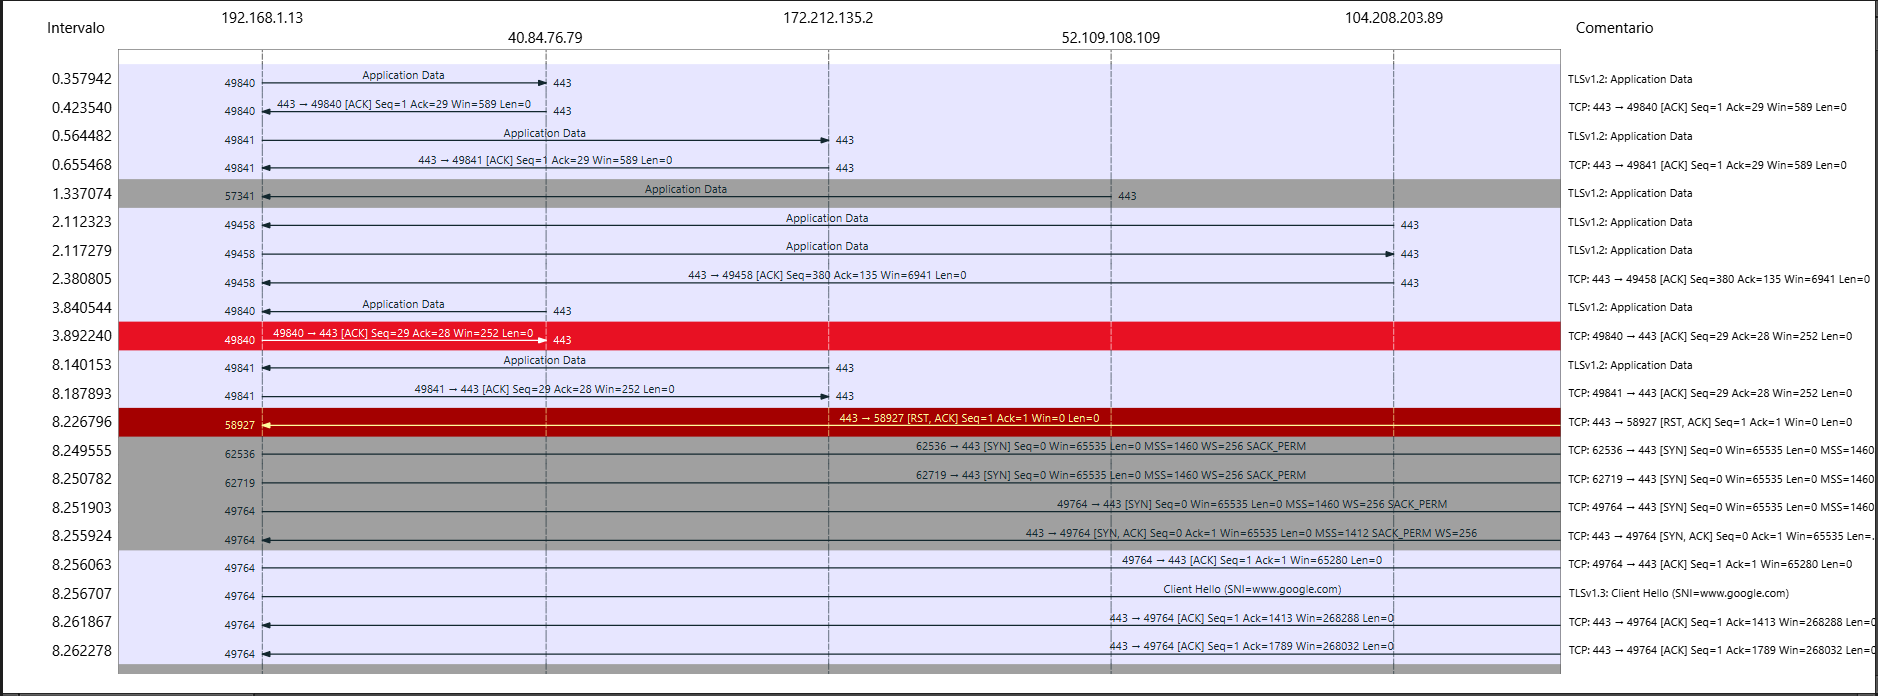
\includegraphics[width=0.95\textwidth]{lab-02-screenshots/8.5-YouTube-flow.png}
    \caption{Flujo de comunicación durante la navegación en YouTube. Se aprecian múltiples \texttt{Application Data} (tráfico cifrado) y \texttt{ACKs} propios de TCP hacia distintos hosts de Google/YouTube.}
\end{figure}

\begin{figure}[H]
    \centering
    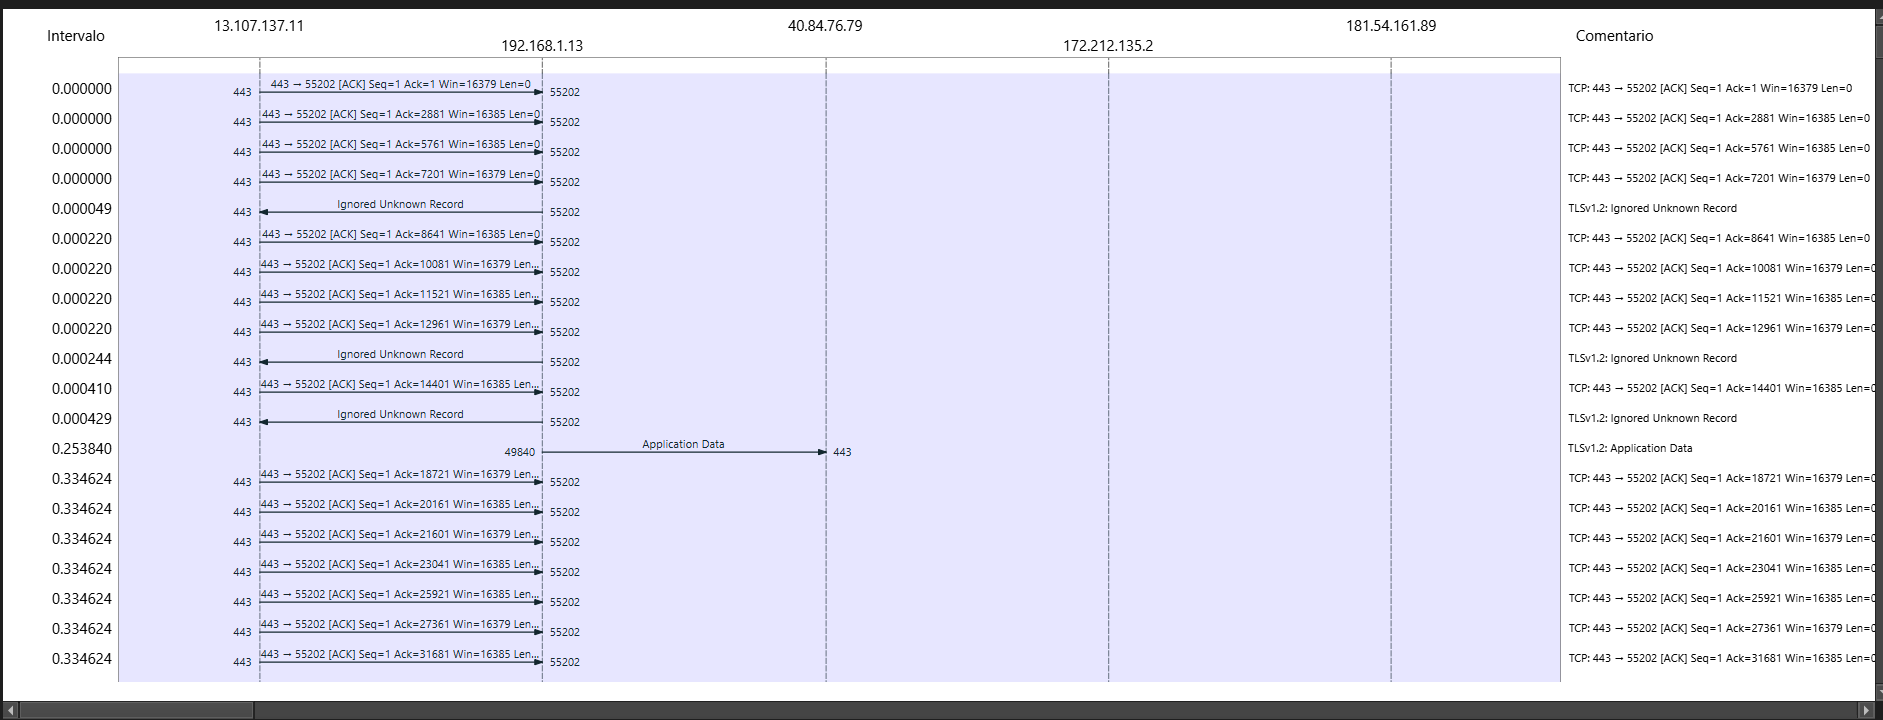
\includegraphics[width=0.95\textwidth]{lab-02-screenshots/8.5-HTTPS-flow.png}
    \caption{Flujo durante la navegación en sitios HTTPS (El Espectador, El Tiempo, Uniandes y Bancolombia). Se observa el establecimiento de conexión (SYN/SYN-ACK/ACK) y el posterior \textit{handshake TLS} (por ejemplo, \textit{Client Hello}).}
\end{figure}

%==============================================================
%=================== Evidencia de Capas =======================
%==============================================================
\subsection*{Análisis de la Capa de Aplicación (TLS)}

Durante el \textit{handshake TLS}, el cliente envía un \texttt{Client Hello} indicando versiones soportadas (TLS 1.2/1.3), \textit{cipher suites} y el nombre del servidor (\textit{SNI}). 
El servidor responde con \texttt{Server Hello} seleccionando parámetros criptográficos y entrega su \textit{Certificate} (X.509) para autenticación. 
Tras la negociación de claves, la sesión opera con \texttt{Application Data} (HTTP cifrado).

\begin{figure}[H]
    \centering
    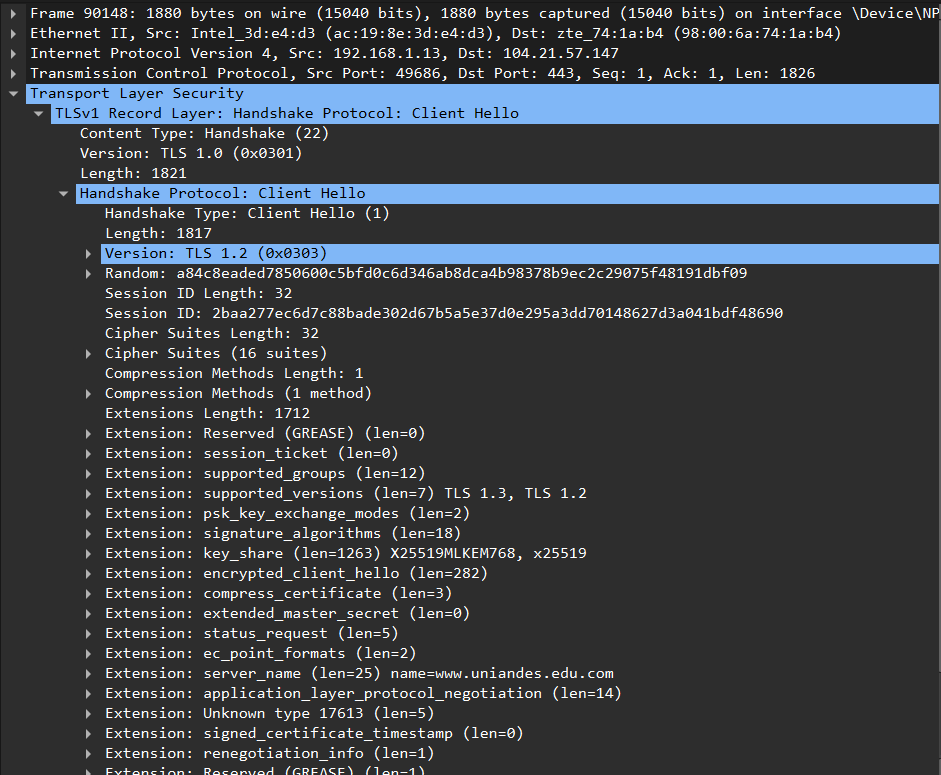
\includegraphics[width=0.9\textwidth]{lab-02-screenshots/8.5-CapaAplicacion-HTTPS.png}
    \caption{\texttt{Client Hello} hacia \texttt{www.uniandes.edu.co}. Se observan extensiones TLS (p.\,ej., \textit{supported\_versions}, \textit{server\_name}).}
\end{figure}

\begin{figure}[H]
    \centering
    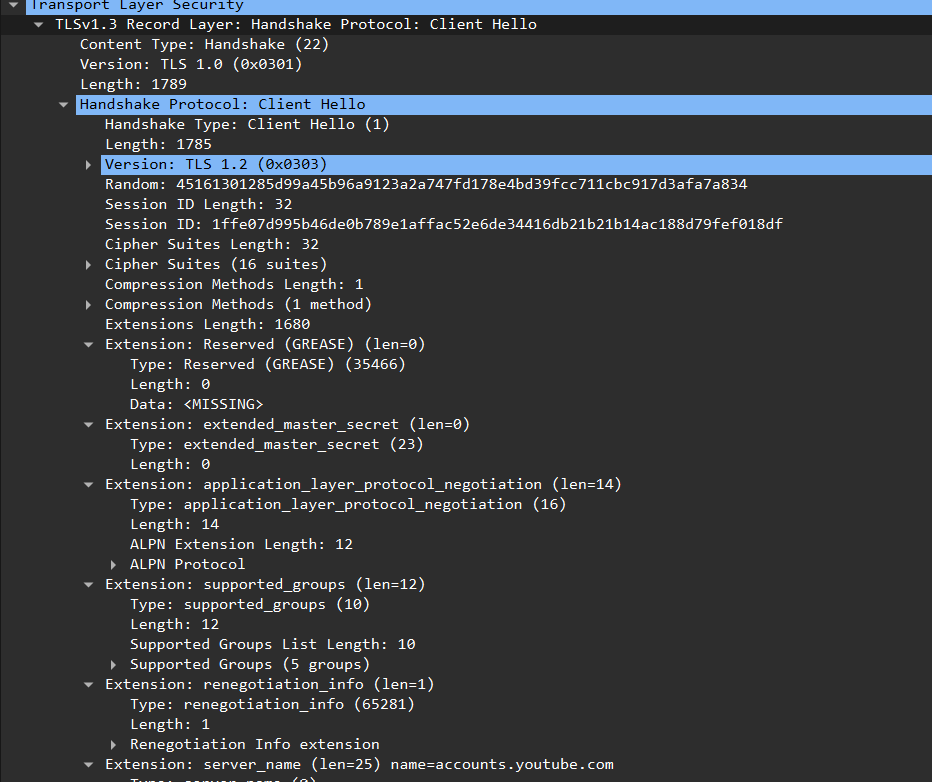
\includegraphics[width=0.9\textwidth]{lab-02-screenshots/8.5-CapaAplicacion-Youtube.png}
    \caption{\texttt{Client Hello} hacia \texttt{accounts.youtube.com}. Se evidencia el uso de TLS 1.2/1.3, \textit{cipher suites} ofrecidas y el SNI del host.}
\end{figure}

\noindent\textit{Implicación:} la capa de aplicación expone la negociación TLS, pero el contenido HTTP queda cifrado.

%--------------------------------------------------------------
\subsection*{Análisis de la Capa de Transporte (TCP)}

HTTPS requiere de TCP para asegurar fiabilidad (entrega ordenada, control de congestión) y se inicia con el \textit{three-way handshake} (SYN, SYN-ACK, ACK). 
En las capturas se aprecian campos como puertos origen/destino, números de secuencia, ventana y flags (\texttt{PSH}, \texttt{ACK}), además del \textit{payload} que TLS cifra.

\begin{figure}[H]
    \centering
    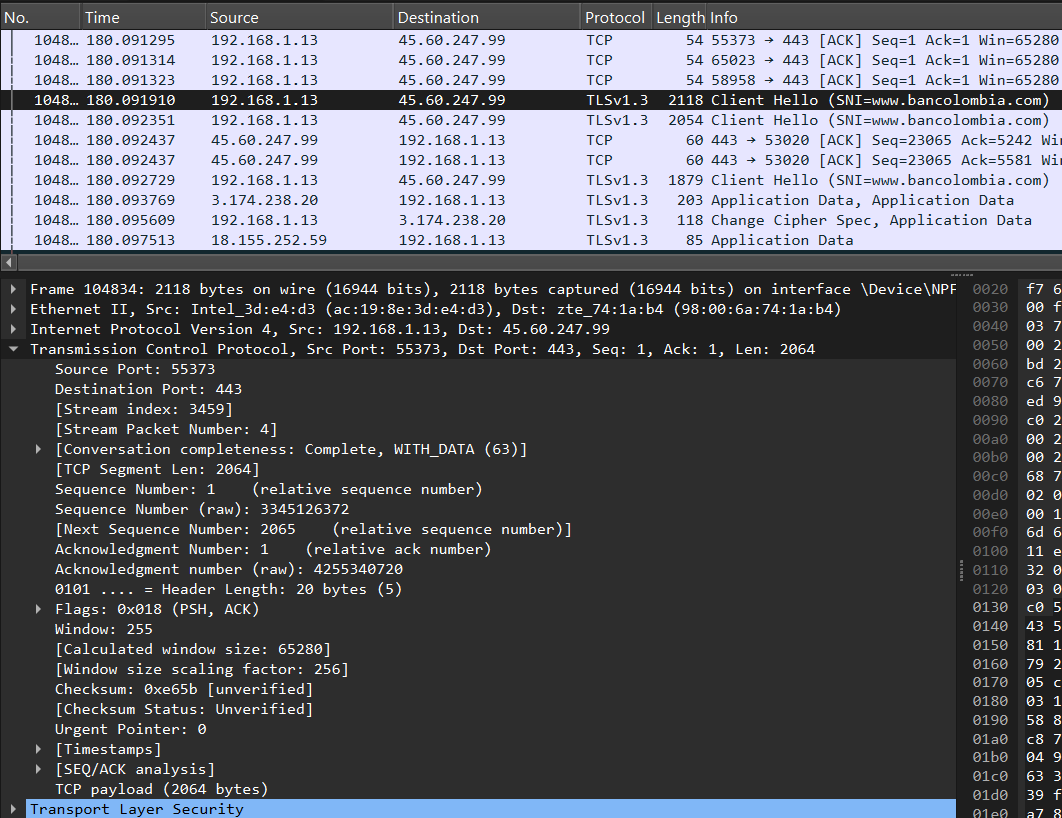
\includegraphics[width=0.9\textwidth]{lab-02-screenshots/8.5-CapaTransporte-HTTPS.png}
    \caption{Detalle TCP hacia \texttt{www.bancolombia.com}: puertos, números de secuencia/ack, ventana y \texttt{TCP payload} (transportado por TLS).}
\end{figure}

\begin{figure}[H]
    \centering
    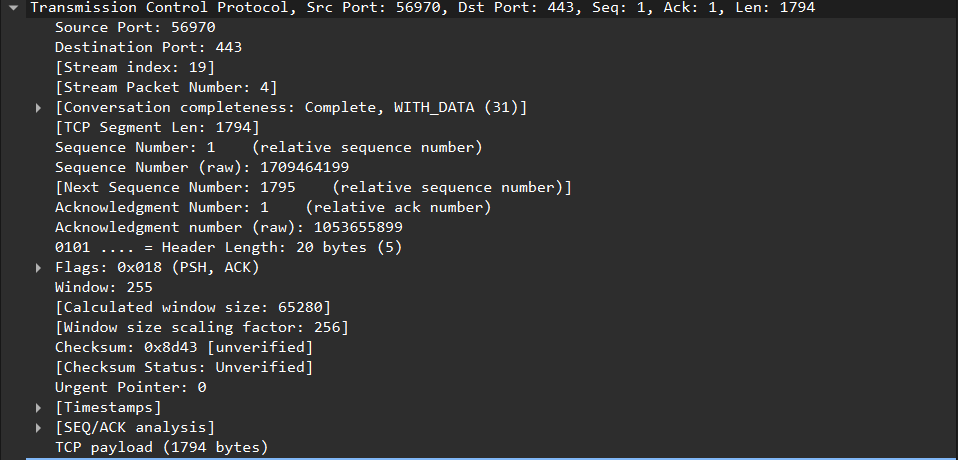
\includegraphics[width=0.9\textwidth]{lab-02-screenshots/8.5-CapaTransporte-Youtube.png}
    \caption{Paquete TCP en conexión a YouTube mostrando longitud de segmento, flags y \texttt{TCP payload}; el contenido de aplicación va cifrado por TLS.}
\end{figure}

%==============================================================
%=================== Evidencia por Sitio ======================
%==============================================================
\subsection*{Evidencia de paquetes HTTPS por sitio web}

\begin{figure}[H]
    \centering
    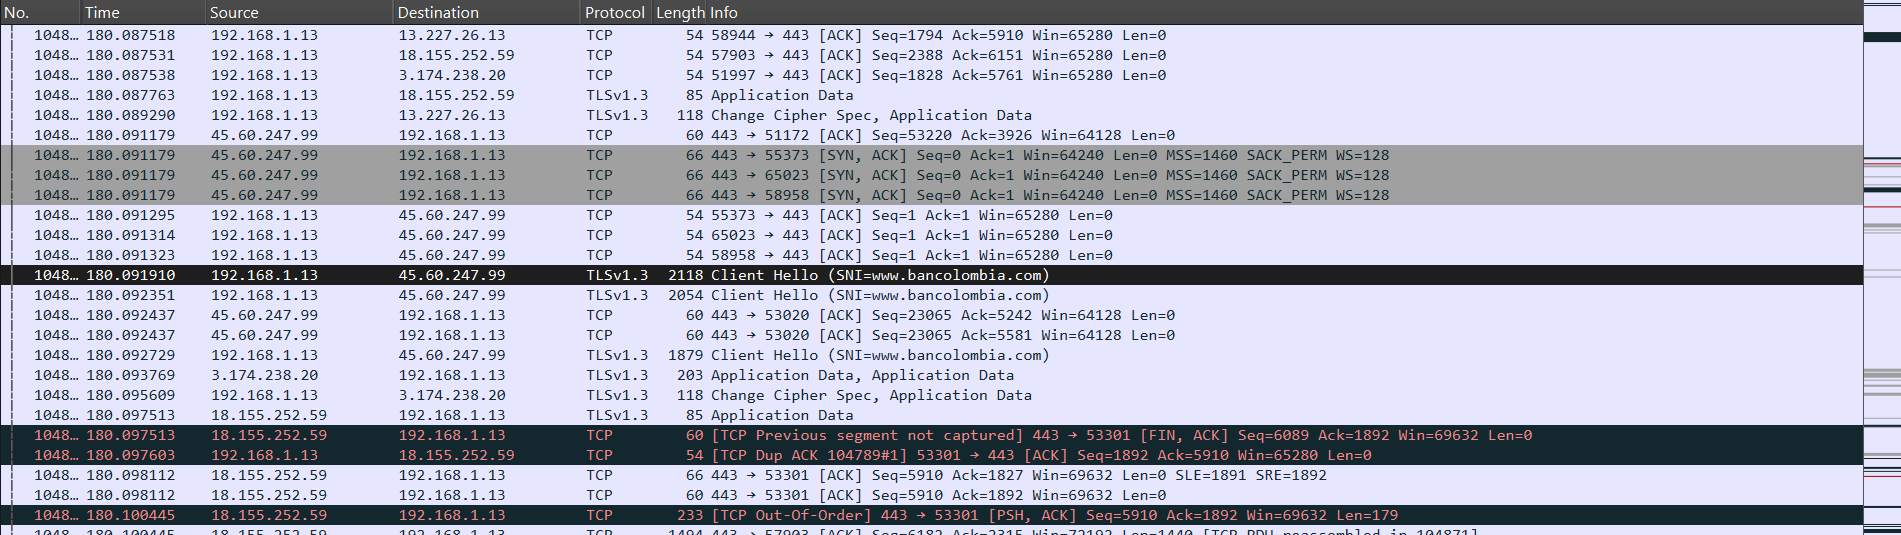
\includegraphics[width=0.95\textwidth]{lab-02-screenshots/8.5-HTTPS-bancolombia.png}
    \caption{\texttt{Client Hello} hacia \texttt{www.bancolombia.com} (TLS 1.3). Evidencia del inicio del \textit{handshake} y establecimiento de un canal cifrado adecuado para datos financieros.}
\end{figure}

\begin{figure}[H]
    \centering
    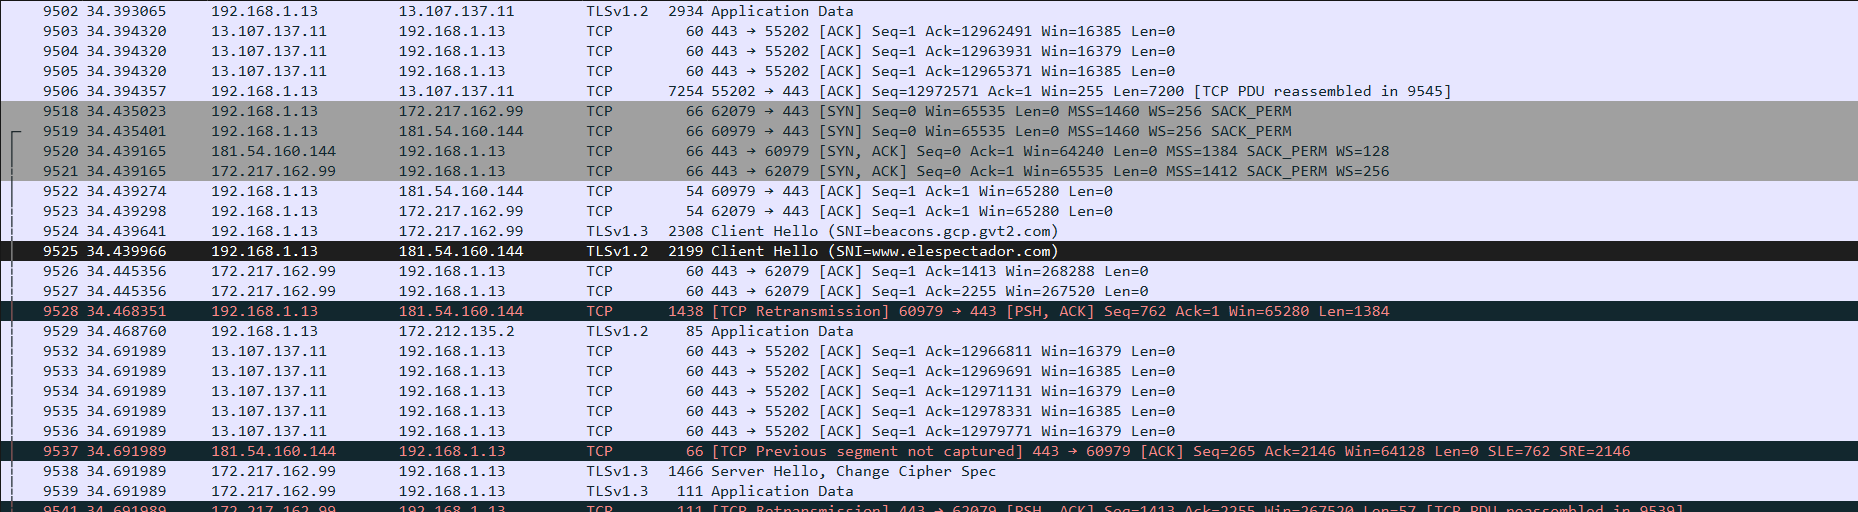
\includegraphics[width=0.95\textwidth]{lab-02-screenshots/8.5-HTTPS-elespectador.png}
    \caption{Conexión a \texttt{www.elespectador.com}. Se visualiza \texttt{Client Hello} (TLS 1.2) y, a continuación, \texttt{Application Data} (HTTP sobre TLS).}
\end{figure}

\begin{figure}[H]
    \centering
    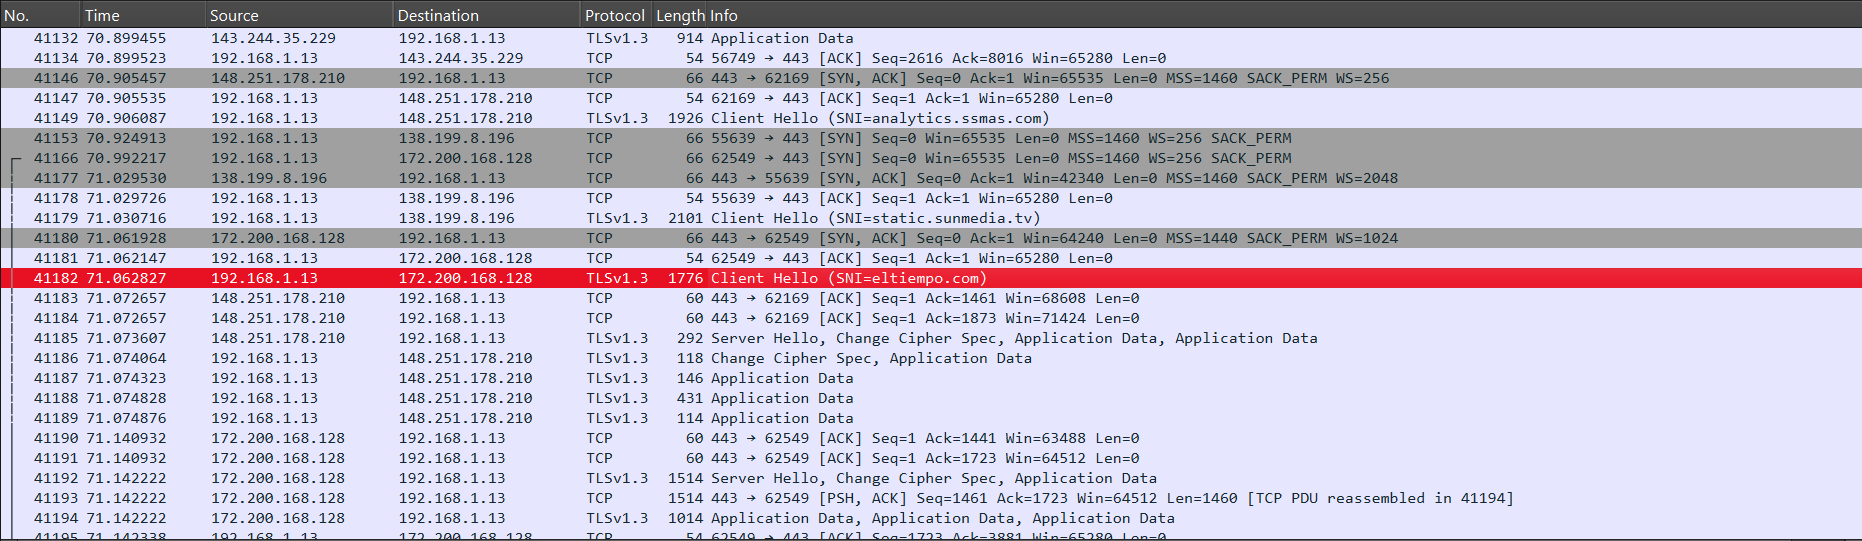
\includegraphics[width=0.95\textwidth]{lab-02-screenshots/8.5-HTTPS-eltiempo.png}
    \caption{Tráfico hacia \texttt{www.eltiempo.com}: \texttt{Client Hello} en TLS 1.3 seguido de \texttt{Server Hello}/\texttt{Change Cipher Spec} y \texttt{Application Data}.}
\end{figure}

\begin{figure}[H]
    \centering
    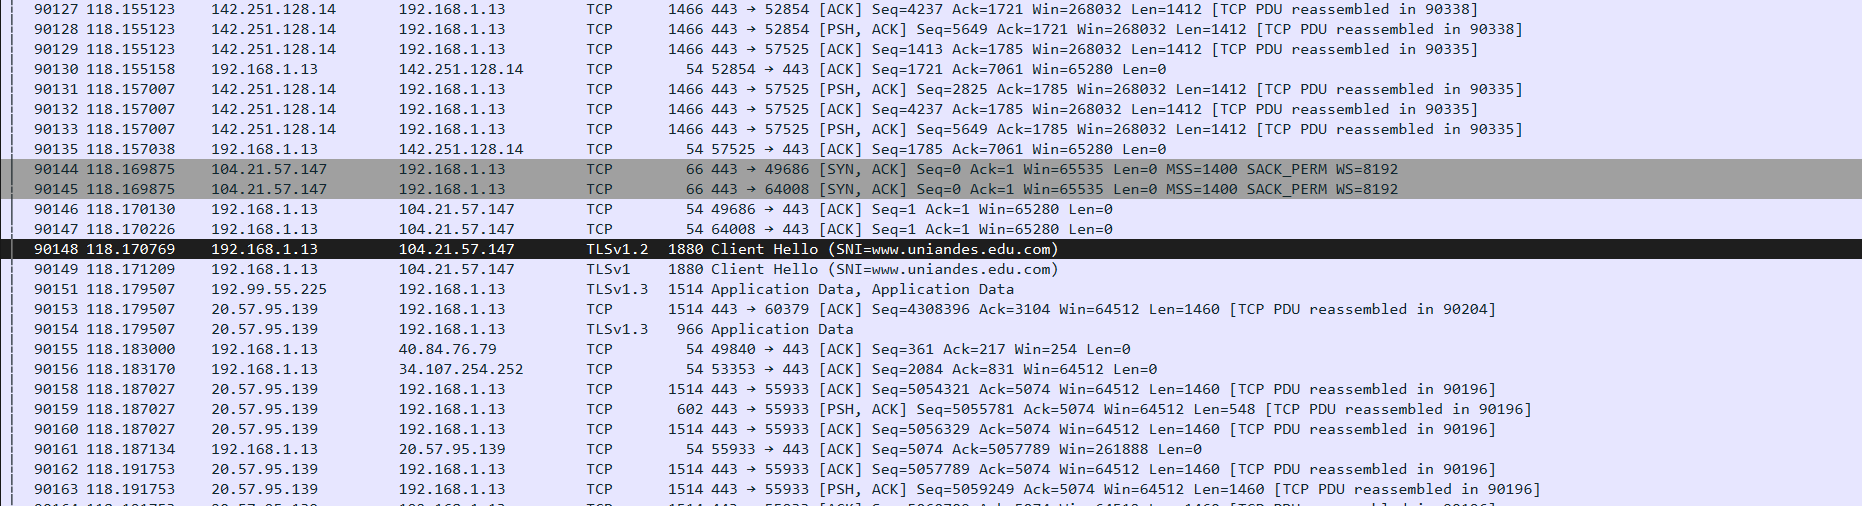
\includegraphics[width=0.95\textwidth]{lab-02-screenshots/8.5-HTTPS-uniandes.png}
    \caption{Tráfico hacia \texttt{www.uniandes.edu.co}. Evidencia de \texttt{Client Hello} con SNI del host y negociación de versiones/cifrados.}
\end{figure}

%--------------------------------------------------------------
\subsection*{Evidencia de paquetes en YouTube}

\begin{figure}[H]
    \centering
    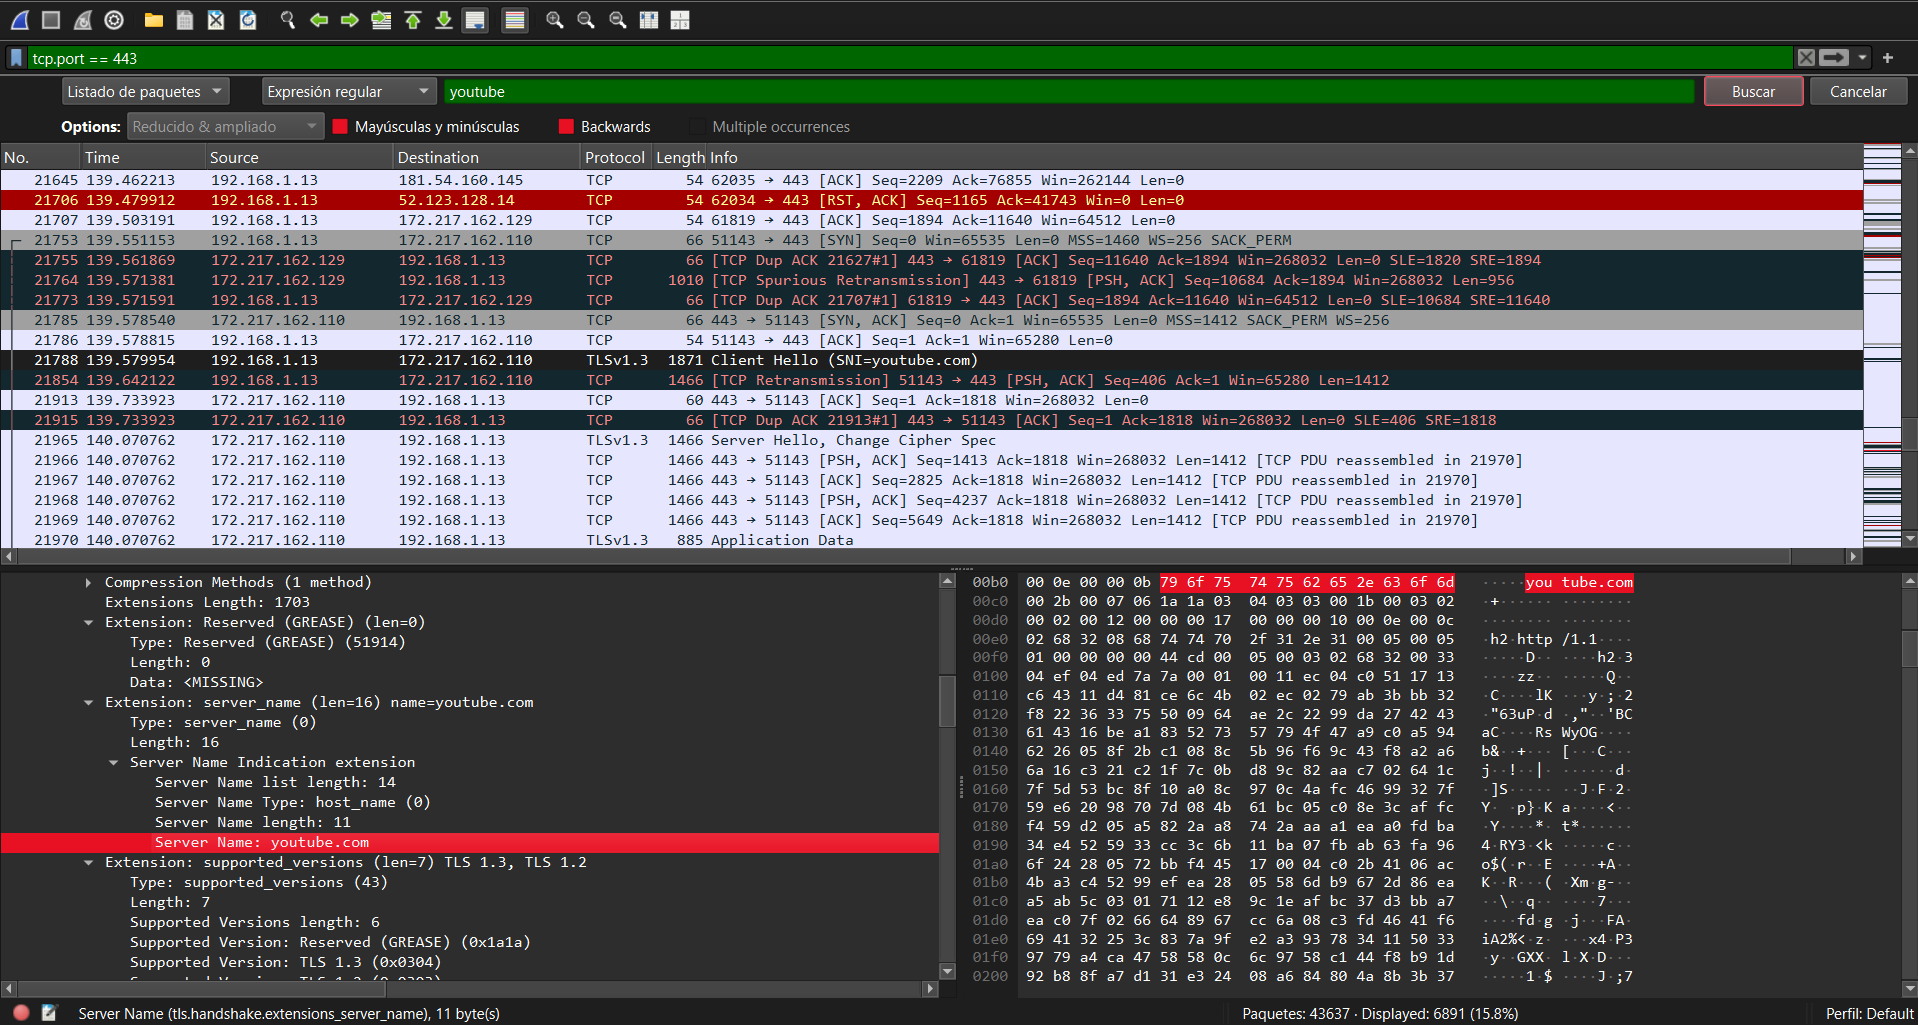
\includegraphics[width=0.95\textwidth]{lab-02-screenshots/8.5-Packets-Youtube.png}
    \caption{Listado filtrado por \texttt{tcp.port == 443} con conexiones a \texttt{youtube.com}. Se observan \textit{handshake TLS} y posteriormente \texttt{Application Data}.}
\end{figure}

\begin{figure}[H]
    \centering
    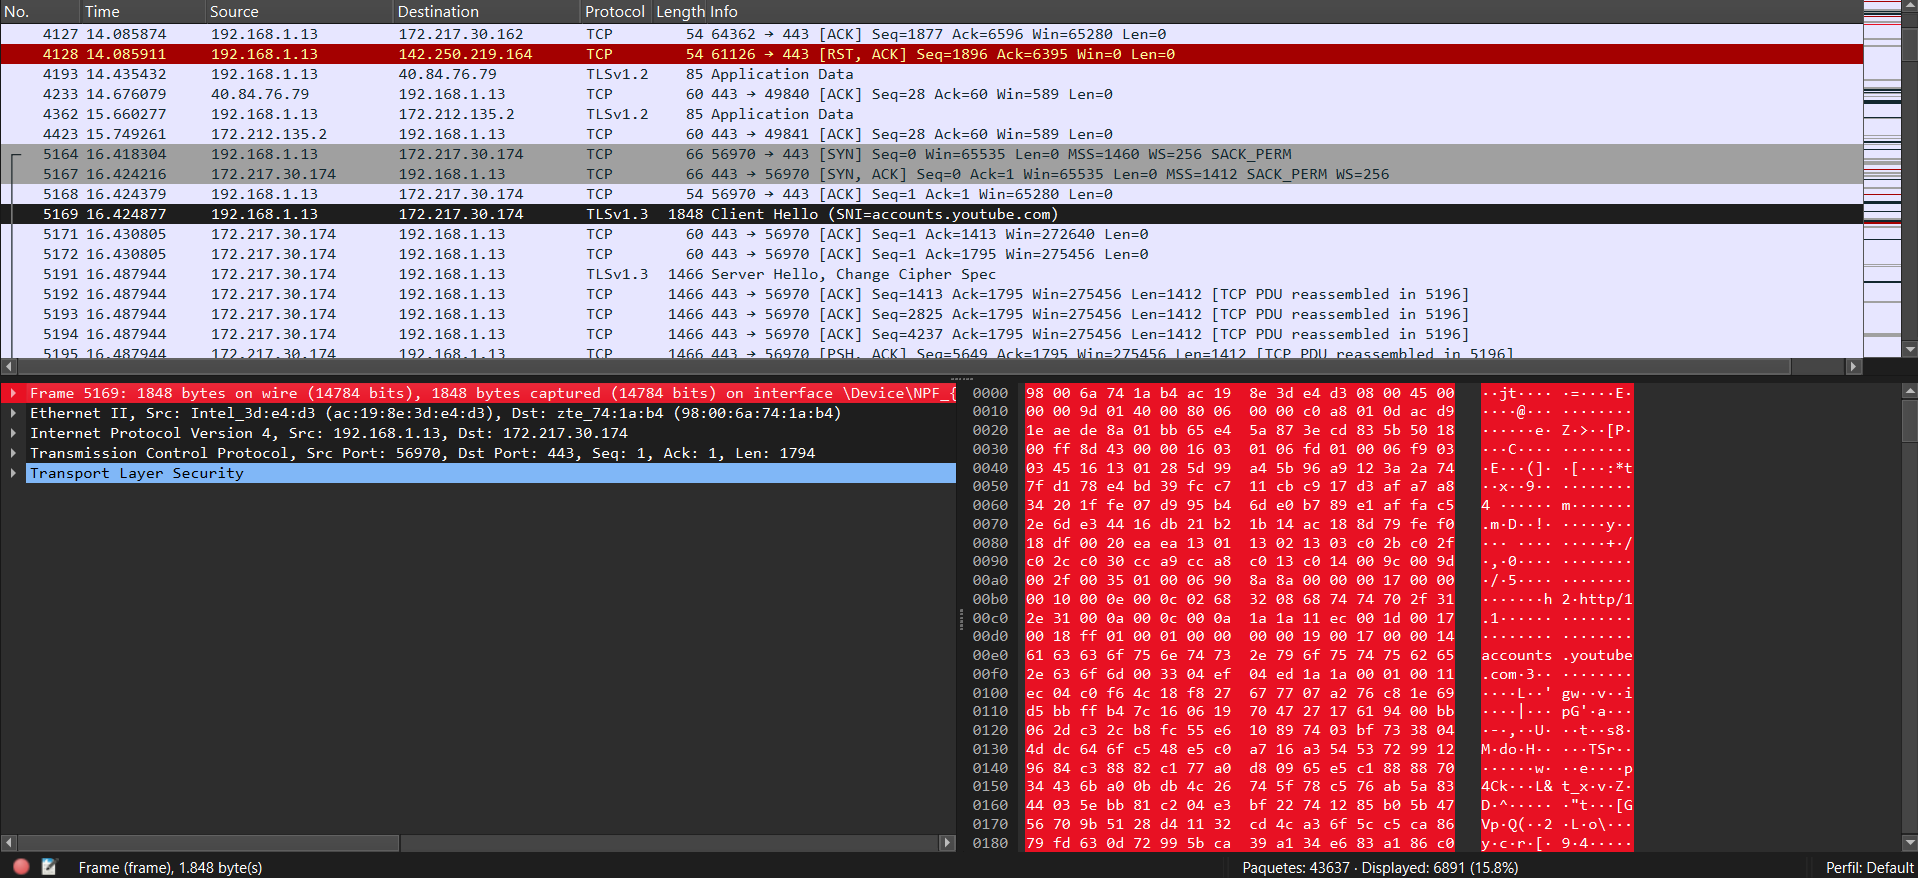
\includegraphics[width=0.95\textwidth]{lab-02-screenshots/8.5-Paquete-Youtube.png}
    \caption{Detalle de un paquete TLS asociado a YouTube: la capa de aplicación aparece como \texttt{Application Data}, confirmando el cifrado del contenido HTTP.}
\end{figure}

%==============================================================
%======================= Tablas (opc) =========================
%==============================================================
\subsection*{Ejemplos de paquetes (tabla)}
% Requiere \usepackage{array} si deseas columnas con p{..}
\begin{table}[H]
\centering
\caption{Ejemplos representativos de paquetes capturados (YouTube)}
\begin{tabular}{|c|c|c|c|c|}
\hline
\textbf{Fuente} & \textbf{Destino} & \textbf{Protocolo} & \textbf{Puerto Origen} & \textbf{Puerto Destino} \\
\hline
192.168.1.13 & \textit{YouTube/Google IP} & TCP (TLS 1.3) & \textit{efímero} & 443 \\
192.168.1.13 & \textit{YouTube/Google IP} & TCP (TLS 1.2) & \textit{efímero} & 443 \\
\hline
\end{tabular}
\end{table}

\begin{table}[H]
\centering
\caption{Ejemplos representativos de paquetes (otros sitios HTTPS)}
\begin{tabular}{|c|c|c|c|c|}
\hline
\textbf{Fuente} & \textbf{Destino} & \textbf{Protocolo} & \textbf{Puerto Origen} & \textbf{Puerto Destino} \\
\hline
192.168.1.13 & \textit{bancolombia.com (IP)} & TCP (TLS 1.3) & \textit{efímero} & 443 \\
192.168.1.13 & \textit{uniandes.edu.co (IP)} & TCP (TLS 1.2/1.3) & \textit{efímero} & 443 \\
\hline
\end{tabular}
\end{table}

%==============================================================
%==================== Cierre/Análisis =========================
%==============================================================
\subsection*{Conclusiones generales}
\begin{itemize}
    \item HTTPS combina HTTP con TLS sobre TCP/443, garantizando \textbf{confidencialidad}, \textbf{integridad} y \textbf{autenticación} del servidor mediante certificados X.509.
    \item Las capturas muestran el \textbf{handshake TLS} (\texttt{Client Hello}, \texttt{Server Hello}, \texttt{Certificate}) seguido de \texttt{Application Data} (HTTP cifrado), por lo cual el contenido de aplicación no es legible.
    \item El uso de TCP evidencia control de fiabilidad (SYN/SYN-ACK/ACK, números de secuencia, ventanas y \texttt{ACKs}).
    \item En YouTube se observan múltiples flujos cifrados (\texttt{Application Data}) por la naturaleza de \textit{streaming} y recursos; en los demás sitios se confirma el mismo patrón de seguridad.
\end{itemize}



%==============================================================
%=====================   8.6  ================================
%==============================================================
\renewcommand{\thesection}{8.\arabic{section}}
\section{Análisis del protocolo VoIP}
\subsection{Establecimiento de la llamada}


%==============================================================
%=====================   8.7   ================================
%==============================================================
\renewcommand{\thesection}{8.\arabic{section}}
\section{Análisis del protocolo RTMP}
\subsection{Inicio de la transmisión}


%==============================================================
%=====================   8.7   ================================
%==============================================================
\renewcommand{\thesection}{9.\arabic{section}}
\setcounter{section}{0}
\section{Topología}












\begin{thebibliography}{9}


  \bibitem{kurose_ross}
  Computer Networking, a top-down approach. James Kurose, Keith Ross. Addison-Wesley, 6th ed.

  \end{thebibliography}


\end{document}